% A bigon-free dichotomy for pseudoline arrangements: standalone article for Hexagon.
% pdfLaTeX. Compile: latexmk -pdf article.tex (or tectonic -X compile article.tex).
\documentclass[11pt,a4paper]{amsart}
\usepackage[T1]{fontenc}
\usepackage[utf8]{inputenc}
\usepackage{lmodern,microtype,amssymb,mathtools,enumitem,booktabs}
\usepackage[margin=2.7cm]{geometry}
\usepackage{tikz}
\usepackage[hidelinks]{hyperref}
\tikzset{lab/.style={inner sep=0.5pt,font=\scriptsize},
  dot/.style={circle,fill,inner sep=0pt,minimum size=3.2pt}}

\newtheorem{theorem}{Theorem}
\newtheorem{proposition}[theorem]{Proposition}
\newtheorem{lemma}[theorem]{Lemma}
\newtheorem{corollary}[theorem]{Corollary}
\theoremstyle{definition}
\newtheorem{definition}[theorem]{Definition}
\newtheorem{example}[theorem]{Example}
\theoremstyle{remark}
\newtheorem{remark}[theorem]{Remark}

\newcommand{\II}[1]{\mathrm{II}_{#1}}
\newcommand{\IIp}{\mathrm{II}'_{3,2}}
\newcommand{\III}{\mathrm{III}_{6}}
\newcommand{\A}{\mathcal A}
\newcommand{\fac}[1]{\href{https://grothendieck.umontpellier.fr/#1.pdf}{folder~#1}}

\title[A bigon-free dichotomy]{A bigon-free dichotomy for pseudoline arrangements,\\ after a note of Grothendieck}
\author{Michel Hua}
\address{Commutator, Paris, France}
\email{michel@commutator.io}
\thanks{ORCID 0009-0002-8304-0683.}
\date{7 November 2026}
\subjclass[2020]{52C30; 52C40, 05C10}
\keywords{pseudoline arrangements, Sylvester--Gallai, near-pencil, complete quadrangle, generalised maps, Lean}



\begin{document}
\begin{abstract}
A pseudoline of an arrangement in the real projective plane is \emph{bigonal} when it carries exactly two vertices of the arrangement. In an undated folder of working notes from the early 1980s, Grothendieck states that every arrangement without bigonal pseudolines is either four pseudolines in general position or contains one of three configurations: five pseudolines in general position, a pencil of three and a pencil of two without the line joining their centres, or the complete quadrangle. The notes derive this from a statement that is false as written, and they give no independent proof. We give a short proof, together with the ordering of the pseudolines that the notes ask for, and we deduce that for $n \ge 6$ the near-pencils are the only arrangements of $n$ pseudolines containing none of the three configurations. The dichotomy has been checked by an exhaustive enumeration of all arrangements of at most nine pseudolines, and it is formalised in the proof assistant Lean for a combinatorial model of arrangements, generalised maps of Euler characteristic one.
\end{abstract}

\maketitle

\section{Introduction}

An \emph{arrangement of pseudolines} is a finite family of at least three simple closed curves in the real projective plane, none of them separating it, any two of which meet in exactly one point, where they cross, and not all passing through one point \cite{grunbaum1972,felsnergoodman2017}. Arrangements of straight lines are the first examples. The \emph{vertices} are the points where at least two pseudolines meet. We call a pseudoline \emph{bigonal} when it carries exactly two vertices, so that every other pseudoline meets it at one of these two points; an arrangement is \emph{bigon-free} when none of its pseudolines is bigonal. Since every pseudoline meets the others, it carries at least one vertex, and it carries exactly one only in a pencil, which is excluded; so \emph{bigon-free} means that every pseudoline carries at least three vertices.

Four configurations will be used throughout (Figure~\ref{fig:four}):
\begin{itemize}[leftmargin=2.2em]
\item[$\II4$] four pseudolines in general position, that is, no three through a point;
\item[$\II5$] five pseudolines in general position;
\item[$\IIp$] five pseudolines $a, b, c, d, e$, where $a, b, c$ pass through a point $p$, the pseudolines $d, e$ do not, and $d \cap e$ lies on none of $a, b, c$; so $\{a,b,c\}$ is the only concurrent triple, and none of the five passes through both $p$ and $d \cap e$;
\item[$\III$] the complete quadrangle: the six pseudolines joining four points $P_1, \dots, P_4$ pairwise, each passing through exactly two of them.
\end{itemize}
A \emph{sub-arrangement} is a subfamily of at least three pseudolines, with the vertices it determines; we say that $\A$ \emph{contains} a configuration when some sub-arrangement of $\A$ is of that type.

\begin{figure}[ht]
\centering
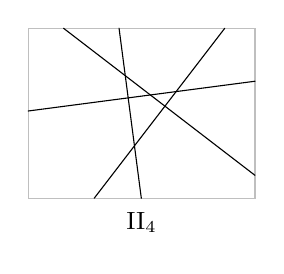
\begin{tikzpicture}[scale=0.72,line cap=round,baseline=0pt]
  \draw[black!25] (0,0) rectangle (4,3);
  \draw (0,1.54) -- (4,2.065);
  \draw (1.163,0) -- (3.467,3);
  \draw (1.602,3) -- (1.995,0);
  \draw (0.622,3) -- (4,0.405);
  \node[below,font=\small,text height=1.8ex,text depth=0.6ex] at (2,0) {$\II4$};
\end{tikzpicture}\quad
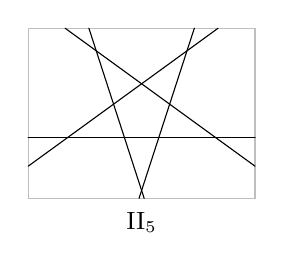
\begin{tikzpicture}[scale=0.72,line cap=round,baseline=0pt]
  \draw[black!25] (0,0) rectangle (4,3);
  \draw (3.349,3.000) -- (0.000,0.567);
  \draw (1.070,3.000) -- (2.045,0.000);
  \draw (0.000,1.079) -- (4.000,1.079);
  \draw (1.955,0.000) -- (2.930,3.000);
  \draw (4.000,0.567) -- (0.651,3.000);
  \node[below,font=\small,text height=1.8ex,text depth=0.6ex] at (2,0) {$\II5$};
\end{tikzpicture}\quad
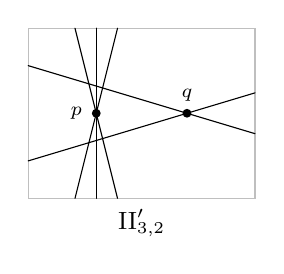
\begin{tikzpicture}[scale=0.72,line cap=round,baseline=0pt]
  \draw[black!25] (0,0) rectangle (4,3);
  \draw (0.825,0) -- (1.575,3);
  \draw (0.825,3) -- (1.575,0);
  \draw (1.2,0) -- (1.2,3);
  \draw (0,0.66) -- (4,1.86);
  \draw (0,2.34) -- (4,1.14);
  \node[dot] at (1.2,1.5) {};
  \node[dot] at (2.8,1.5) {};
  \node[lab] at (0.85,1.5) {$p$};
  \node[lab] at (2.8,1.82) {$q$};
  \node[below,font=\small,text height=1.8ex,text depth=0.6ex] at (2,0) {$\IIp$};
\end{tikzpicture}\quad
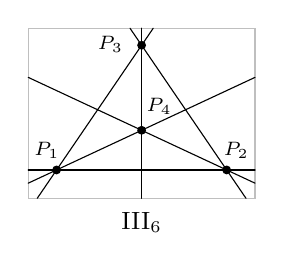
\begin{tikzpicture}[scale=0.72,line cap=round,baseline=0pt]
  \draw[black!25] (0,0) rectangle (4,3);
  \draw (0,0.5) -- (4,0.5);
  \draw (0.159,0) -- (2.205,3);
  \draw (0,0.267) -- (4,2.133);
  \draw (1.795,3) -- (3.841,0);
  \draw (0,2.133) -- (4,0.267);
  \draw (2,0) -- (2,3);
  \node[dot] at (0.5,0.5) {};
  \node[dot] at (3.5,0.5) {};
  \node[dot] at (2,2.7) {};
  \node[dot] at (2,1.2) {};
  \node[lab] at (0.33,0.85) {$P_1$};
  \node[lab] at (3.67,0.85) {$P_2$};
  \node[lab] at (1.45,2.72) {$P_3$};
  \node[lab] at (2.31,1.62) {$P_4$};
  \node[below,font=\small,text height=1.8ex,text depth=0.6ex] at (2,0) {$\III$};
\end{tikzpicture}
\caption{The four configurations, drawn with straight lines in an affine chart in which every crossing is visible. In $\IIp$ no line of the five passes through both $p$ and $q$.}\label{fig:four}
\end{figure}

\subsection*{The source}
The University of Montpellier holds the mathematical papers that Alexandre Grothendieck left to Jean Malgoire, and publishes their facsimiles. Its \fac{80}, \emph{Systèmes de pseudo-droites}, is undated in his hand; the archival inventory dates it from 1981 onwards, and an administrative notice of 13 May 1981 used as scrap paper on page~27 agrees. Pages~20 to~28 look for the arrangements that he calls \emph{crucial} and name them; the four configurations above are among them, with $\II4$, $\II5$, $\III$ in his notation. Page~24 states, boxed, that every arrangement without bigons is either of type $\II4$ or contains one of three types, which are $\II5$, $\III$ and a pencil of three with a pencil of two, written $\mathrm{I}'_{3,2}$; we write $\IIp$. Page~20 announces the same statement with the three configurations drawn, and page~28 states a lemma on the order in which the pseudolines can be added, of which only a sketch is written.

The notes derive the boxed statement from a theorem on the same page, which, as written, is false (Section~\ref{sec:p24}). We have found no independent proof on the pages, and we have not found the statement in print, in Grünbaum's monograph \cite{grunbaum1972} or in the survey of Felsner and Goodman \cite{felsnergoodman2017}. It is elementary, and may be known to specialists. This note records a proof (Theorem~\ref{thm:main}), the ordering of page~28 (Theorem~\ref{thm:order}), a consequence (Corollary~\ref{cor:near}), a computer check, and a formalisation in Lean. The statement is Grothendieck's; the proofs, the corollary, the check and the formalisation are ours.

\section{The dichotomy}

The proof uses one external result, the pseudoline form of the Sylvester--Gallai theorem. A \emph{near-pencil} is an arrangement in which all pseudolines but one pass through a point; a \emph{simple crossing} is a vertex on exactly two pseudolines.

\begin{theorem}[Kelly--Rottenberg {\cite[Th.~3.6]{kellyrottenberg1972}}]\label{thm:sg}
An arrangement of $n$ pseudolines has at least $3n/7$ simple crossings. In particular it has one.
\end{theorem}

The existence of one simple crossing also follows from Melchior's equality, which holds for pseudolines \cite[Th.~1.3]{bokowskipokora2017}; we return to it in Section~\ref{sec:verif}.

We shall often use that two distinct pseudolines meet only once: if a pseudoline passes through two distinct points of another, the two are equal.

\begin{lemma}\label{lem:quad}
A bigon-free arrangement contains four pseudolines in general position.
\end{lemma}

\begin{proof}
Let $\A$ be bigon-free. By Theorem~\ref{thm:sg} it has a simple crossing $p = a \cap b$. Since $a$ is not bigonal it carries vertices $q_1, \dots, q_k$ other than $p$, with $k \ge 2$. A pseudoline $c \ne a$ through some $q_i$ is not $b$ (otherwise $q_i = a \cap b = p$) and misses $p$, which is on $a$ and $b$ only.

Take $c \ni q_i$ and $d \ni q_j$ with $i \ne j$, both different from $a$. If $c \cap b \ne d \cap b$, the four pseudolines $a, b, c, d$ are in general position: $a \cap b = p$ is on neither $c$ nor $d$; $a \cap c = q_i$ and $a \cap d = q_j$ are distinct; $b \cap c$ and $b \cap d$ are distinct; and these are the four triples.

Suppose then that $c \cap b = d \cap b$ for all such choices. Then all the pseudolines other than $a$ through the points $q_i$ meet $b$ at one point $r$: two of them through different points $q_i$, $q_j$ are compared directly, and two through the same $q_i$ are both compared with a pseudoline other than $a$ through some $q_j$, $j \ne i$, which exists since $k \ge 2$ and every vertex lies on at least two pseudolines. If $q_i$ were on two of them, both would pass through $q_i$ and $r$, which are distinct since $r \in b$ and $q_i \notin b$; so they would be equal. Hence $q_i$ lies on $a$ and on exactly one other pseudoline $c_i$. Every pseudoline other than $a, b$ meets $a$ at a point other than $p$, that is, at some $q_i$, so it is one of the $c_i$. Thus $\A = \{a, b, c_1, \dots, c_k\}$, and $b$ carries only $p$ and $r$: it is bigonal, which is excluded.
\end{proof}

\begin{figure}[ht]
\centering
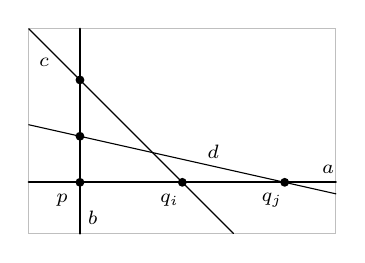
\begin{tikzpicture}[scale=0.65,line cap=round]
\draw[black!25] (0,0) rectangle (6,4);
\draw[thick] (0,1.0) -- (6,1.0);
\draw[thick] (1.0,0) -- (1.0,4);
\draw[] (0,4.0) -- (4.0,0);
\draw[] (0,2.125) -- (6,0.775);
\node[dot] at (1.000,1.000) {};
\node[lab] at (0.65,0.65) {$p$};
\node[dot] at (3.000,1.000) {};
\node[lab] at (2.75,0.65) {$q_i$};
\node[dot] at (5.000,1.000) {};
\node[lab] at (4.75,0.65) {$q_j$};
\node[dot] at (1.000,3.000) {};
\node[dot] at (1.000,1.900) {};
\node[lab] at (5.85,1.25) {$a$};
\node[lab] at (1.25,0.3) {$b$};
\node[lab] at (0.3,3.35) {$c$};
\node[lab] at (3.6,1.6) {$d$};
\end{tikzpicture}\qquad
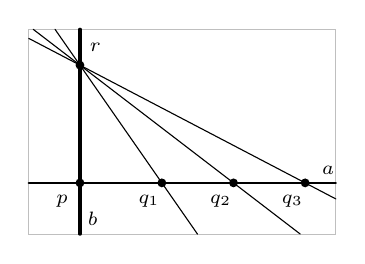
\begin{tikzpicture}[scale=0.65,line cap=round]
\draw[black!25] (0,0) rectangle (6,4);
\draw[thick] (0,1.0) -- (6,1.0);
\draw[very thick] (1.0,0) -- (1.0,4);
\draw[] (0.513,4) -- (3.296,0);
\draw[] (0.087,4) -- (5.304,0);
\draw[] (0,3.823) -- (6,0.686);
\node[dot] at (1.000,1.000) {};
\node[lab] at (0.65,0.65) {$p$};
\node[dot] at (1.000,3.300) {};
\node[lab] at (1.3,3.65) {$r$};
\node[dot] at (2.600,1.000) {};
\node[lab] at (2.35,0.65) {$q_1$};
\node[dot] at (4.000,1.000) {};
\node[lab] at (3.75,0.65) {$q_2$};
\node[dot] at (5.400,1.000) {};
\node[lab] at (5.15,0.65) {$q_3$};
\node[lab] at (5.85,1.25) {$a$};
\node[lab] at (1.25,0.3) {$b$};
\end{tikzpicture}
\caption{The proof of Lemma~\ref{lem:quad}. Left: $c \ni q_i$ and $d \ni q_j$ meet $b$ at different points, and $a, b, c, d$ are in general position. Right: every pseudoline other than $a$ through a $q_i$ passes through the same point $r$ of $b$; then $b$ carries only $p$ and $r$, and is bigonal.}\label{fig:quad}
\end{figure}


Let $Q = \{x, y, z, w\}$ be four pseudolines in general position. Its six vertices are the points $x \cap y$, and two of them are \emph{opposite} when the two pairs are disjoint, as $x \cap y$ and $z \cap w$; there are three opposite pairs. Two vertices that are not opposite lie on a common pseudoline of $Q$.

\begin{lemma}\label{lem:fifth}
Let $\ell \notin Q$ be a pseudoline of $\A$. Then $\ell$ passes through at most two vertices of $Q$, and through two only if they are opposite. If $\ell$ passes through no vertex of $Q$, then $Q \cup \{\ell\}$ is a $\II5$; if it passes through exactly one, then $Q \cup \{\ell\}$ is a $\IIp$.
\end{lemma}

\begin{proof}
If $\ell$ passed through two vertices on a common pseudoline $s$ of $Q$, it would meet $s$ twice and be equal to it. Any three vertices contain two that are not opposite. If $\ell$ passes through no vertex, no three of the five are concurrent. If it passes only through $x \cap y$, then $x, y, \ell$ pass through $p = x \cap y$; $z$ and $w$ miss $p$, since $Q$ is in general position; and $z \cap w$ is on neither $x$ nor $y$, nor on $\ell$, which passes through no other vertex of $Q$.
\end{proof}

A pseudoline through two opposite vertices of $Q$ is a \emph{diagonal} of $Q$. Two diagonals through the same opposite pair meet twice, so they are equal: $Q$ has at most three diagonals in $\A$.

\begin{theorem}[Grothendieck, {\fac{80}}, pp.~20 and~24]\label{thm:main}
A bigon-free arrangement of pseudolines either is $\II4$ or contains $\II5$, $\IIp$ or $\III$.
\end{theorem}

\begin{proof}
Let $\A$ be bigon-free, $Q = \{x,y,z,w\} \subseteq \A$ in general position (Lemma~\ref{lem:quad}), and suppose that $\A$ contains neither $\II5$ nor $\IIp$. By Lemma~\ref{lem:fifth}, every pseudoline of $\A \smallsetminus Q$ is a diagonal of $Q$. If there is none, $\A = Q$ is $\II4$. If there is exactly one, $\delta$ through $x \cap y$ and $z \cap w$, then $\delta$ meets every other pseudoline of $\A = Q \cup \{\delta\}$ at one of these two points, and is bigonal. If there are at least two, say $\delta_1$ through $P_1 = x \cap y$ and $P_2 = z \cap w$, and $\delta_2$ through $P_3 = x \cap z$ and $P_4 = y \cap w$, then the six pseudolines $x, y, z, w, \delta_1, \delta_2$ pass through the pairs $\{P_1, P_3\}$, $\{P_1, P_4\}$, $\{P_2, P_3\}$, $\{P_2, P_4\}$, $\{P_1, P_2\}$, $\{P_3, P_4\}$, and through no other $P_i$, since $Q$ is in general position and each diagonal meets $Q$ only at its two vertices. They form a $\III$.
\end{proof}

\begin{figure}[ht]
\centering
\newcommand{\Qlines}{%
  \draw[black!25] (0,0) rectangle (4,3);
  \draw (0.159,0) -- (2.205,3);
  \draw (0,2.133) -- (4,0.267);
  \draw (0,0.267) -- (4,2.133);
  \draw (1.795,3) -- (3.841,0);
  \node[dot] at (0.5,0.5) {};
  \node[dot] at (3.5,0.5) {};
  \node[dot] at (2,2.7) {};
  \node[dot] at (2,1.2) {};
  \node[dot] at (1.224,1.562) {};
  \node[dot] at (2.776,1.562) {};}
\begin{tikzpicture}[scale=0.72,line cap=round,baseline=0pt]
\Qlines
\draw[dashed,thick] (0,0.9) -- (4,0.9);
\node[lab] at (3.75,1.12) {$\ell$};
\node[below,font=\small,text height=1.8ex,text depth=0.6ex] at (2,0) {$\II5$};
\end{tikzpicture}\quad
\begin{tikzpicture}[scale=0.72,line cap=round,baseline=0pt]
\Qlines
\draw[dashed,thick] (0,1.2) -- (4,1.2);
\node[lab] at (2,0.84) {$P_4$};
\node[lab] at (3.75,1.42) {$\ell$};
\node[below,font=\small,text height=1.8ex,text depth=0.6ex] at (2,0) {$\IIp$};
\end{tikzpicture}\quad
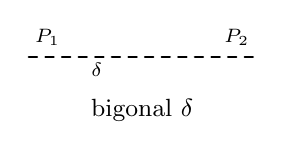
\begin{tikzpicture}[scale=0.72,line cap=round,baseline=0pt]
\Qlines
\draw[dashed,thick] (0,0.5) -- (4,0.5);
\node[lab] at (0.33,0.85) {$P_1$};
\node[lab] at (3.67,0.85) {$P_2$};
\node[lab] at (1.2,0.27) {$\delta$};
\node[below,font=\small,text height=1.8ex,text depth=0.6ex] at (2,0) {bigonal $\delta$};
\end{tikzpicture}\quad
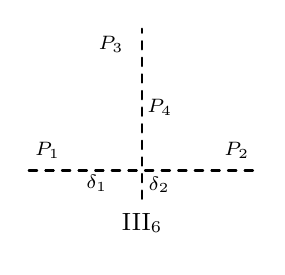
\begin{tikzpicture}[scale=0.72,line cap=round,baseline=0pt]
\Qlines
\draw[dashed,thick] (0,0.5) -- (4,0.5);
\draw[dashed,thick] (2.0,0) -- (2.0,3);
\node[lab] at (0.33,0.85) {$P_1$};
\node[lab] at (3.67,0.85) {$P_2$};
\node[lab] at (1.45,2.72) {$P_3$};
\node[lab] at (2.31,1.62) {$P_4$};
\node[lab] at (1.2,0.27) {$\delta_1$};
\node[lab] at (2.3,0.25) {$\delta_2$};
\node[below,font=\small,text height=1.8ex,text depth=0.6ex] at (2,0) {$\III$};
\end{tikzpicture}
\caption{Lemma~\ref{lem:fifth} and the proof of Theorem~\ref{thm:main}. The four solid pseudolines form $Q$, in general position, with its six vertices; $P_1, P_2$, then $P_3, P_4$, then the two unlabelled vertices are its three opposite pairs. From left to right: a fifth pseudoline $\ell$ through no vertex of $Q$ gives a $\II5$, and one through exactly one vertex gives a $\IIp$; a single diagonal $\delta$, through $P_1$ and $P_2$, meets every other pseudoline at one of these two points and is bigonal; a second diagonal, through $P_3$ and $P_4$, completes the quadrangle $\III$.}\label{fig:diag}
\end{figure}


None of the four alternatives can be omitted. $\II4$, $\II5$ and $\IIp$ are bigon-free (in $\IIp$, each of $a, b, c$ carries $p$ and its points on $d$ and $e$, and each of $d, e$ carries $d \cap e$ and three more), and so is $\III$, each of whose sides carries two of the $P_i$ and its point on the opposite side. And $\III$ contains neither $\II5$ nor $\IIp$: deleting the side $P_1P_2$ leaves two concurrent triples, at $P_3$ and at $P_4$, and every five sides arise this way.

\begin{corollary}\label{cor:five}
The bigon-free arrangements of five pseudolines are $\II5$ and $\IIp$. Hence a bigon-free arrangement other than $\II4$ contains a bigon-free arrangement of five pseudolines, or a complete quadrangle.
\end{corollary}

\begin{proof}
A bigon-free arrangement of five pseudolines is not $\II4$ and cannot contain a $\III$, so by Theorem~\ref{thm:main} it contains, and therefore is, a $\II5$ or a $\IIp$; both are bigon-free.
\end{proof}

\section{The ordering of page 28}

Page~28 asks for a numbering $D_1, \dots, D_n$ of the pseudolines, starting from a $\II4$ or a $\III$, such that no $D_i$ is bigonal in the partial arrangement $\{D_1, \dots, D_i\}$. We prove a stronger form.

\begin{theorem}\label{thm:order}
The pseudolines of a bigon-free arrangement $\A$ can be numbered $D_1, \dots, D_n$ so that either $D_1, \dots, D_4$ form a $\II4$ or $D_1, \dots, D_6$ form a $\III$, and so that every partial arrangement $\{D_1, \dots, D_i\}$ from there on is bigon-free.
\end{theorem}

\begin{proof}
Adding a pseudoline never removes a vertex from the pseudolines already present. So it suffices that each pseudoline, when it is added, meets the earlier ones in at least three distinct points.

A pseudoline $\ell$ outside a $\III$ meets its six sides in at least three points. Indeed, a point lies on at most three sides, and only the $P_i$ lie on three, since any three sides include two with a common $P_i$, and these meet only there. Two of the $P_i$ share a side, so two points lie on at most five sides. If $\A$ contains a $\III$, start from it and add the other pseudolines in any order.

Otherwise, let $Q \subseteq \A$ be in general position (Lemma~\ref{lem:quad}). By Lemma~\ref{lem:fifth}, a pseudoline outside $Q$ meets $Q$ in at least three points unless it is a diagonal of $Q$, and $\A$ has at most one diagonal $\delta$ of $Q$, since two would form a $\III$ with $Q$. Start from $Q$, add the pseudolines other than $\delta$ in any order, and add $\delta$ last: then all its vertices are present, and there are at least three since $\A$ is bigon-free.
\end{proof}

\section{Arrangements avoiding the three configurations}

\begin{corollary}\label{cor:near}
Let $n \ge 6$. An arrangement of $n$ pseudolines contains none of $\II5$, $\IIp$, $\III$ if and only if it is a near-pencil.
\end{corollary}

\begin{proof}
A near-pencil contains none of them: it has a single vertex on more than two pseudolines, while $\III$ has four, and any five of its pseudolines include at least four through the centre, while $\II5$ has no concurrent triple and $\IIp$ has two pseudolines off its triple point.

Conversely, let $\A$ contain none of the three. It is not $\II4$, since $n \ge 6$, so by Theorem~\ref{thm:main} it has a bigonal pseudoline $D$, with vertices $P$ and $Q$. Every other pseudoline passes through exactly one of them, since $D$ is the only pseudoline through both. Let $s$ and $t$ be the numbers of pseudolines other than $D$ through $P$ and through $Q$, so $s + t = n - 1 \ge 5$. If $s \ge 3$ and $t \ge 2$, three pseudolines $a, b, c \ne D$ through $P$ and two $d, e \ne D$ through $Q$ form a $\IIp$: $d \cap e = Q$ lies on none of $a, b, c$, and $P$ on neither $d$ nor $e$. The case $s \ge 2$, $t \ge 3$ is symmetric. Since $s + t \ge 5$, the remaining cases are $\min(s, t) \le 1$. If $t = 1$, the $s + 1 = n - 1$ pseudolines through $P$ (with $D$) and the one other pseudoline through $Q$ form a near-pencil, and similarly if $s = 1$. The case $t = 0$ is excluded, since then all pseudolines pass through $P$.
\end{proof}

\begin{figure}[ht]
\centering
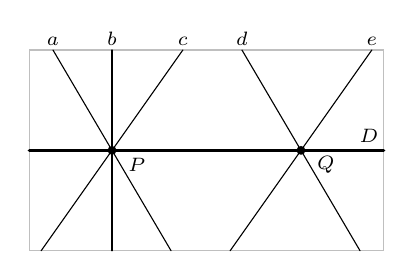
\begin{tikzpicture}[scale=0.75,line cap=round]
\draw[black!25] (0,0) rectangle (6,3.4);
\draw[very thick] (0,1.7) -- (6,1.7);
\draw (0.4,3.4) -- (2.4,0);
\draw (1.4,0) -- (1.4,3.4);
\draw (0.2,0) -- (2.6,3.4);
\draw (3.6,3.4) -- (5.6,0);
\draw (3.4,0) -- (5.8,3.4);
\node[dot] at (1.4,1.7) {};
\node[lab] at (1.82,1.45) {$P$};
\node[dot] at (4.6,1.7) {};
\node[lab] at (5.02,1.45) {$Q$};
\node[lab] at (5.75,1.95) {$D$};
\foreach \x/\n in {0.4/a,1.4/b,2.6/c,3.6/d,5.8/e} \node[above,inner sep=1.5pt,font=\scriptsize] at (\x,3.4) {$\n$};
\end{tikzpicture}
\caption{The proof of Corollary~\ref{cor:near}: a bigonal pseudoline $D$, with $s$ pseudolines through $P$ and $t$ through $Q$. Here $s = 3$ and $t = 2$, and the five thin pseudolines form a $\IIp$.}\label{fig:cor}
\end{figure}


For $n = 4$ the arrangements avoiding the three configurations are $\II4$ and the near-pencil, and for $n = 5$ the near-pencil and the arrangement of two pencils of three sharing a pseudoline; these small cases agree with the enumeration below.

\section{The statement of page 24 as written}\label{sec:p24}

The theorem from which page~24 derives the boxed statement assumes that there are no two vertices such that every pseudoline passes through one of them, and that the arrangement contains no $\II5$, and concludes that it is a complete quadrangle $\III$ or a complete quadrilateral with its three diagonals, $\mathrm{IV}_7$. Six straight lines already refute it.

\begin{example}\label{ex:p24}
Let $A = (0,0)$, $B = (1,0)$, $C = (0,1)$ in the affine plane, and take the six lines
\[
\begin{gathered}AB\colon y = 0,\quad BC\colon x + y = 1,\quad CA\colon x = 0,\\ a\colon y = 2x,\quad b\colon y = 3x - 3,\quad c\colon y = 5x + 1,\end{gathered}
\]
the last three passing through $A$, $B$ and $C$. Writing a line $u_0x + u_1y + u_2z = 0$ of the projective plane as an integer triple, three lines are concurrent if and only if the determinant of their triples vanishes. Of the twenty triples, exactly three vanish, $\{AB, CA, a\}$, $\{AB, BC, b\}$ and $\{BC, CA, c\}$, concurrent at $A$, $B$, $C$. Two vertices carry at most five of the six lines, since two of the triple points share a side; every five lines contain a concurrent triple; and there are three triple points, not the four of $\III$, and six lines, not the seven of $\mathrm{IV}_7$ (Figure~\ref{fig:cex}).
\end{example}

\begin{figure}[ht]
\centering
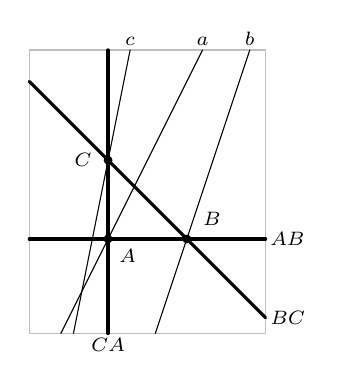
\begin{tikzpicture}[scale=1,line cap=round]
\draw[black!25] (0,0) rectangle (3.0,3.6);
\draw[very thick] (0,1.2) -- (3.0,1.2);
\draw[very thick] (0,3.2) -- (3.0,0.2);
\draw[very thick] (1.0,0) -- (1.0,3.6);
\draw (0.4,0) -- (2.2,3.6);
\draw (1.6,0) -- (2.8,3.6);
\draw (0.56,0) -- (1.28,3.6);
\node[dot] at (1,1.2) {};
\node[lab] at (1.25,0.98) {$A$};
\node[dot] at (2,1.2) {};
\node[lab] at (2.32,1.45) {$B$};
\node[dot] at (1,2.2) {};
\node[lab] at (0.68,2.2) {$C$};
\node[above,inner sep=1.5pt,font=\scriptsize] at (1.28,3.6) {$c$};
\node[above,inner sep=1.5pt,font=\scriptsize] at (2.2,3.6) {$a$};
\node[above,inner sep=1.5pt,font=\scriptsize] at (2.8,3.6) {$b$};
\node[below,inner sep=1.5pt,font=\scriptsize] at (1,0) {$CA$};
\node[right,inner sep=1.5pt,font=\scriptsize] at (3,1.2) {$AB$};
\node[right,inner sep=1.5pt,font=\scriptsize] at (3,0.2) {$BC$};
\end{tikzpicture}
\caption{The six lines of Example~\ref{ex:p24}: the triangle $ABC$ (thick) and one more line through each vertex. Some crossings lie outside the chart.}\label{fig:cex}
\end{figure}


The example contains a $\IIp$ (the five lines $AB$, $CA$, $a$, $b$, $c$ have the single concurrent triple $\{AB, CA, a\}$), so it does not contradict Theorem~\ref{thm:main}. Nor does $\mathrm{IV}_7$, which contains a $\IIp$ as well: two sides $x, y$ of the quadrilateral and the three diagonals have the single concurrent triple formed by $x$, $y$ and the diagonal through $x \cap y$ (the three diagonals are not concurrent, since the Fano matroid is not orientable \cite{bjorner1999}).

The theorem of page~24 becomes true once $\IIp$ is excluded together with $\II5$, and $\mathrm{IV}_7$ is then dropped from its conclusion. Its hypothesis implies that the arrangement is bigon-free, since the two vertices of a bigonal pseudoline would be met by every pseudoline. The proof of Theorem~\ref{thm:main} then shows that the arrangement consists of four pseudolines $Q$ in general position and some of their diagonals. With no diagonal, or one, two vertices of $Q$ meet every pseudoline; with three, it is $\mathrm{IV}_7$, which contains a $\IIp$. So it has exactly two diagonals and is a $\III$.

\section{Verification}\label{sec:verif}

\subsection*{Enumeration}
All arrangements of $n \le 9$ pseudolines were enumerated, simple or not, as reorientation classes of rank-$3$ oriented matroids whose underlying matroid is simple \cite{bjorner1999}, and the simple ones up to $n = 10$. The method is single-element extension with pruning by the three-term Grassmann--Plücker relations, and a canonical form computed on the flag graph of the cell decomposition of the sphere. The counts of classes, $1, 2, 4, 17, 143, 4890, 461053$ for $n = 3, \dots, 9$, and $4382$ and $312356$ simple ones for $n = 9, 10$, agree with the known values \cite{finschifukuda2003}. All $466094$ bigon-free arrangements with $n \le 9$ ($461049$ of them with $n = 9$), and all $312356$ simple ones with $n = 10$, satisfy Theorem~\ref{thm:main} and the strong ordering of Theorem~\ref{thm:order}. A deletion-closed search of the arrangements containing none of the three configurations finds only the near-pencils for $6 \le n \le 16$, as Corollary~\ref{cor:near} predicts. The hypothesis is weak: at $n = 9$, all but four arrangements are bigon-free, and all but $4382$ of the bigon-free ones (the simple arrangements) were found to contain a $\IIp$.

\subsection*{Formalisation}
Theorem~\ref{thm:main} is formalised in Lean~4 with the Mathlib library, for a combinatorial model of arrangements that page~60 of the folder describes: a map, topological or combinatorial, whose underlying surface is a real projective plane. A map of a possibly non-orientable surface is a \emph{generalised map} \cite{lienhardt1994}: a finite set of flags with three fixed-point-free involutions $\alpha_0, \alpha_1, \alpha_2$, with $\alpha_0\alpha_2$ a fixed-point-free involution; vertices, edges and faces are the orbits of $\langle\alpha_1, \alpha_2\rangle$, $\langle\alpha_0, \alpha_2\rangle$, $\langle\alpha_0, \alpha_1\rangle$, and the Euler characteristic is $\chi = V - E + F$. A combinatorial arrangement labels the flags by pseudolines, constantly on edges, so that each pseudoline is connected and passes exactly once through each of its vertices, every vertex lies on at least two pseudolines, two pseudolines meet at exactly one vertex, and $\chi = 1$. The axioms do not require the pseudolines to go straight at a vertex, so the formal theorem is slightly more general than the statement for maps. Figure~\ref{fig:gmap} shows the three involutions near an edge.

\begin{figure}[ht]
\centering
\begin{tikzpicture}[scale=1.5,line cap=round,>=stealth]
\tikzset{flag/.style={circle,draw,fill=white,inner sep=0pt,minimum size=4.5pt}}
\draw[thick] (-1.0,0) -- (4.0,0);
\draw (0,-1.0) -- (0,1.2);
\draw (3,-1.0) -- (3,1.2);
\node[dot] at (0,0) {};
\node[dot] at (3,0) {};
\node[lab] at (-0.2,-0.2) {$v$};
\node[lab] at (3.2,-0.2) {$w$};
\node[flag,fill=black] (d) at (0.8,0.25) {};
\node[flag] (d0) at (2.2,0.25) {};
\node[flag] (d2) at (0.8,-0.25) {};
\node[flag] (d1) at (0.25,0.8) {};
\draw[<->,shorten <=2pt,shorten >=2pt] (d) to[bend left=20] node[above,font=\scriptsize] {$\alpha_0$} (d0);
\draw[<->,shorten <=2pt,shorten >=2pt] (d) to[bend left=45] node[right,font=\scriptsize] {$\alpha_2$} (d2);
\draw[<->,shorten <=2pt,shorten >=2pt] (d) to[bend right=30] node[above right,inner sep=1pt,font=\scriptsize] {$\alpha_1$} (d1);
\node[lab] at (0.58,0.17) {$\phi$};
\node[right,font=\scriptsize] at (4.0,0) {$\ell$};
\node[above,font=\scriptsize] at (0,1.2) {$m$};
\node[above,font=\scriptsize] at (3,1.2) {$m'$};
\end{tikzpicture}
\caption{Flags of a generalised map near the edge $vw$, which lies on the pseudoline $\ell$; the crossing pseudolines $m$ and $m'$ pass through $v$ and $w$. A flag $\phi$ (black) is a vertex, an edge and a face, mutually incident. The involution $\alpha_0$ changes only the vertex, $\alpha_1$ only the edge, $\alpha_2$ only the face.}\label{fig:gmap}
\end{figure}

The formal proof follows Section~2, except for Theorem~\ref{thm:sg}, which it replaces by Melchior's counting \cite{melchior1941}, \cite[Th.~1.3]{bokowskipokora2017}: the skeleton of a bigon-free map has no loop and no multiple edge, so every face has at least three sides; with $\chi = 1$ and $E = \sum_v \nu(v)$, where $\nu(v)$ is the number of pseudolines through $v$, this gives $\sum_v (3 - \nu(v)) \ge 3$, hence a simple crossing. The rest is incidence geometry. The proof uses only Lean's standard axioms. It is registered in the Palomar Registry as entry \href{https://palomar-registry.org/entry.html?id=PALOMAR-2026-11-07-000003}{PALOMAR-2026-11-07-000003}, from the repository \href{https://github.com/Commutator-IO/grothendieck-project-palomar}{Commutator-IO/grothendieck-project-palomar} (theorem \texttt{Grothendieck.\allowbreak Folder80Maps2.\allowbreak PseudolineMap.\allowbreak map\_dichotomy}). The ordering (Theorem~\ref{thm:order}), Corollary~\ref{cor:near}, and the passage from a topological arrangement to its map are not formalised.

\section*{Statement on the use of artificial intelligence}
The transcription of folder~80 used here, the search for a proof, the enumeration program, the Lean formalisation and a first draft of this text were produced with language models (Claude Opus~5 and Opus~5.5, Anthropic), under the author's direction. The author checked the proofs, the computations and the references, and takes full responsibility for the content. The formal proof is checked mechanically by Lean. The transcriptions and the enumeration program are in the public repository \href{https://github.com/Commutator-IO/grothendieck-project}{Commutator-IO/grothendieck-project} (directory \texttt{computations/bigon}).

\section*{Acknowledgements}
The facsimiles are published by the University of Montpellier, \href{https://grothendieck.umontpellier.fr/}{grothendieck.umontpellier.fr}.

\begin{thebibliography}{9}
\bibitem{bjorner1999} A.~Björner, M.~Las~Vergnas, B.~Sturmfels, N.~White, G.~M.~Ziegler, \emph{Oriented Matroids}, 2nd ed., Encyclopedia of Mathematics and its Applications~46, Cambridge University Press, 1999, \href{https://doi.org/10.1017/CBO9780511586507}{doi:10.1017/CBO9780511586507}.
\bibitem{bokowskipokora2017} J.~Bokowski, P.~Pokora, On the Sylvester--Gallai and the orchard problem for pseudoline arrangements, \emph{Period.\ Math.\ Hungar.} 77 (2018), 164--174, \href{https://doi.org/10.1007/s10998-017-0224-x}{doi:10.1007/s10998-017-0224-x}.
\bibitem{felsnergoodman2017} S.~Felsner, J.~E.~Goodman, Pseudoline arrangements, in J.~E.~Goodman, J.~O'Rourke, C.~D.~Tóth (eds.), \emph{Handbook of Discrete and Computational Geometry}, 3rd ed., CRC Press, Boca Raton, FL, 2017, ch.~5.
\bibitem{finschifukuda2003} L.~Finschi, K.~Fukuda, Combinatorial generation of small point configurations and hyperplane arrangements, in B.~Aronov et al.\ (eds.), \emph{Discrete and Computational Geometry: The Goodman--Pollack Festschrift}, Algorithms and Combinatorics~25, Springer, 2003, 425--440, \href{https://doi.org/10.1007/978-3-642-55566-4_19}{doi:10.1007/978-3-642-55566-4\_19}.
\bibitem{grunbaum1972} B.~Grünbaum, \emph{Arrangements and Spreads}, CBMS Regional Conference Series in Mathematics~10, American Mathematical Society, 1972.
\bibitem{kellyrottenberg1972} L.~M.~Kelly, R.~Rottenberg, Simple points in pseudoline arrangements, \emph{Pacific J.\ Math.} 40 (1972), 617--622, \href{https://doi.org/10.2140/pjm.1972.40.617}{doi:10.2140/pjm.1972.40.617}.
\bibitem{lienhardt1994} P.~Lienhardt, $N$-dimensional generalized combinatorial maps and cellular quasi-manifolds, \emph{Internat.\ J.\ Comput.\ Geom.\ Appl.} 4 (1994), 275--324, \href{https://doi.org/10.1142/S0218195994000173}{doi:10.1142/S0218195994000173}.
\bibitem{melchior1941} E.~Melchior, Über Vielseite der projektiven Ebene, \emph{Deutsche Math.} 5 (1941), 461--475, Zbl~0025.09105.
\end{thebibliography}

\end{document}
